\chapter{Mathematical Derivations}
\label{sec:proofs}


\section{Simplified equation of motion for diagonal $R$}
\label{sec:Rdiagndof}

Here the derivation of the simplified form of equations of motion, where intrinsic and extrinsic forces are two separate terms, is derived for arbitrary $n$-DoF fully actuated robots.

\paragraph{Assumptions} 

Two assumptions are necessary for this form. First, that a coordinates system can be selected so that the gear-ratio matrix $R$ is diagonal for any selected operating mode:
%
\begin{align}
R_{i,j} = 0 \quad \forall \; i \neq j
\end{align}
%

Second, that dynamic forces related to viscous damping and inertial forces from the rotor side are linear with respect to rotor velocity:
%
\begin{align}
\vec{\tau}_{rotor-inertia} = I \dot{\vec{w}}  \quad  \vec{\tau}_{rotor-damping} = B \vec{w}
\end{align}
%

Note that additionally, in all cases, matrix $I$ and $D$ are diagonal since motor rotors are not coupled directly. 

\paragraph{Derivation}

Starting from the general, eq. XX, the EoM are:
%
\begin{align}
H \vec{ \ddot{q} } + C\vec{ \dot{q} } + D \vec{ \dot{q} } + \vec{ g }
		= R^T  \left[ 
		\vec{ \tau } - I \vec{ \dot{w} } - B \vec{ w }       
		\right]
\end{align}
%
Then substituting motor velocity to joint coordinates using the kinematic relation, eq. XX,
%
\begin{align}
H \vec{ \ddot{q} } + C\vec{ \dot{q} } + D \vec{ \dot{q} } + \vec{ g }
		&= R^T  \left[ 
		\vec{ \tau } - I R \vec{ \ddot{q} } - B R\vec{ \dot{q} }       
		\right] \\
H \vec{ \ddot{q} } + C\vec{ \dot{q} } + D \vec{ \dot{q} } + \vec{ g }
		&= R^T \vec{ \tau } - R^T I R \vec{ \ddot{q} } - R^T B R \vec{ \dot{q} }  
\end{align}
%
Then because $R$, $I$ and $B$ matrix are diagonal, they can be permuted and also $R^T=R$. Hence, the EoM can be rearranged:
%
\begin{align}
H \vec{ \ddot{q} } + C\vec{ \dot{q} } + D \vec{ \dot{q} } + \vec{ g }
		&= R \vec{ \tau } - R R I \vec{ \ddot{q} } - R R B \vec{ \dot{q} }  
\end{align}
%
Then, assuming the robotic system is fully actuated, the R matrix is square and invertible. Then multiplying by $R^{-1}$ from the left on both side:
%
\begin{align}
R^{-1} \left[ H \vec{ \ddot{q} } + C\vec{ \dot{q} } + D \vec{ \dot{q} } + \vec{ g } \right]
		&= \vec{ \tau } - R I \vec{ \ddot{q} } - R B \vec{ \dot{q} }  
\end{align}
%
Then rearranging:
%
\begin{align}
R^{-1} \left[ H \vec{ \ddot{q} } + C\vec{ \dot{q} } + D \vec{ \dot{q} } + \vec{ g } \right]
		&= \vec{ \tau } - R  \left[ I \vec{ \ddot{q} } + B \vec{ \dot{q} }  \right]
\end{align}
%
and thus obtain the desired final form:
%
\begin{align}
\vec{ \tau } &=  R^{-1} \underbrace{ \left[ H \vec{ \ddot{q} } + C\vec{ \dot{q} } + D \vec{ \dot{q} } + \vec{ g } \right] }_{\vec{\tau}_E}
 + R \underbrace{ \left[ I \vec{ \ddot{q} } + B \vec{ \dot{q} }  \right]}_{\vec{\tau}_I}
\end{align}
%



\newpage
\section{Optimal gear-ratio along a known trajectory}
\label{sec:optgearproof}

Starting from the EoM, eq. XXX, assuming that the robot is fully actuated and viscous forces linear in speed, it is possible to derive closed form expression for the optimal gear-ratio.


\subsection{Single DoF}
\label{sec:optgearproof1}

Starting with the EoM in inverse dynamic form (from eq. XXX):
%
\begin{align}
\tau  &=  \frac{\tau_E}{R} + R \tau_I
\end{align}
%
Using a quadratic cost function to minimize:
%
\begin{align}
J &=  \tau^2 = \frac{\tau_E^2}{R^2} + 2 \tau_E \tau_I + R^2 \tau_I^2
\end{align}
%

Finding the gear-ratio that minimize this cost can be formulated as:
%
\begin{align}
R^* &=  \operatornamewithlimits{argmin}\limits_{R} J \\
   &   \text{s.t.} \quad R \in \Re  \quad \& \quad R > 0
\end{align}
%
A non-real value would have no physical sense. A negative $R$ value would be physically possible, for instance the reverse gear in a car. However, for symmetric electric motors, in the sense that they behave the same way for any sign of torque and speed, there should be no gain obtained by changing the direction of the motor velocity. This can be seen as the cost function is symetric with respect to $R$:
%
\begin{align}
J(R) = J( -R )
\end{align}
%

\paragraph{Derivation}

First finding the partial derivative of the cost $J$ with respect to $R$:
%
\begin{align}
\frac{ \partial J }{ \partial R  } &=  2 \tau \frac{ \partial \tau }{ \partial R } = 2 \left( \frac{\tau_E}{R} + R \tau_I \right) \left( -\frac{\tau_E}{R^2} + \tau_I \right) \\
\frac{ \partial J }{ \partial R  } &= 2 \left( R \tau_I^2 - \frac{\tau_E^2}{R^3} \right)
\end{align}
%
Then the second derivative:
%
\begin{align}
\frac{ \partial^2 J }{ \partial R^2  } &= 2 \left( \tau_I^2 + 3 \frac{\tau_E^2}{R^4} \right)
\end{align}
%
Hence, on the domain of interest, the second derivative is always positive:
%
\begin{align}
\frac{ \partial^2 J }{ \partial R^2  } >= 0  \quad \forall \quad R \in (0,+\infty)
\end{align}
%
Thus the cost function $J$ is convex in the desired interval of possible $R$ values. The minimum of the function can thus be found by solving for the point where the first derivative is equal to zero:
%
\begin{align}
0 &= \frac{ \partial J }{ \partial R  } = 2 \left( R \tau_I^2 - \frac{\tau_E^2}{R^3} \right) \\
R \tau_I^2 &= \frac{\tau_E^2}{R^3} 
\end{align}
%
Since $R>0$, it is possible to multiply both side by $R$, leading to
%
\begin{align}
R^4 \tau_I^2 &= \tau_E^2
\end{align}
%
Then, assuming a non-degenerative case of $\tau_I \neq 0$, it leads to
%
\begin{align}
R^4  &= \frac{\tau_E^2}{\tau_I^2} \\
R^2  &= \pm \sqrt{ \frac{\tau_E^2}{\tau_I^2} } = \pm \frac{\tau_E}{\tau_I} \\
R    &= \pm \sqrt{ \pm \frac{\tau_E}{\tau_I} } 
\end{align}
%
Then, the only real and positive solution to this equation is given by:
%
\begin{align}
R    &= \sqrt{ \left| \frac{\tau_E}{\tau_I} \right|} 
\end{align}
%

\paragraph{Solution}

The minimal cost value is thus obtain with the optimal gear-ratio value:
%
\begin{align}
R^*    &= \sqrt{ \left| \frac{\tau_E}{\tau_I} \right|} 
\end{align}
%
Which lead to the minimum cost:
%
\begin{align}
J^*    &=  2 \tau_E \tau_I  + 2 \left| \tau_E \tau_I \right| 
\end{align}
%
Note that the the minimized cost is zero when extrinsic and intrinsic forces have opposite signs.

\paragraph{Degenerative cases}
If the intrinsic forces are equal to zero, then the cost tends towards zero as the gear-ratio $R$ tends toward $\infty$:
%
\begin{align}
\tau_I = 0 \quad \& \quad R \rightarrow \infty \quad \Rightarrow \quad J \rightarrow 0
\end{align}
%
If the extrinsic forces are equal to zero, then the cost tends towards zero as the gear-ratio $R$ tends toward zero:
%
\begin{align}
\tau_E = 0 \quad \& \quad R \rightarrow 0 \quad \Rightarrow \quad J \rightarrow 0
\end{align}
%
If both the extrinsic forces and intrinsic forces are equal to zero, then the cost is zero for any gear-ratio:
%
\begin{align}
\tau_E = 0 \quad \& \quad \tau_I = 0 \quad \Rightarrow \quad J = 0  \quad \forall R
\end{align}
%


\subsection{Multiple DoF}
\label{sec:optgearproofn}

Starting with the EoM in inverse dynamic form (from eq. XXX):
%
\begin{align}
\vec{ \tau } &=  R^{-1} \vec{\tau}_E + R \vec{\tau}_I
\end{align}
%
Using the following quadratic cost function:
%
\begin{align}
J &=  \vec{ \tau }^T \vec{ \tau }
\end{align}
%
Finding the gear-ratios matrix $R$ that minimize this cost can be formulated as
%
\begin{align}
R^* &=  \operatornamewithlimits{argmin}\limits_{R} J \\
    &   \text{s.t.} \quad R_{i,j} \in \Re  \quad \& \quad R_{i,j} > 0  \quad \& \quad 
\end{align}
%

\paragraph{Derivation}

Using index notation, the EoM and cost function can be written as:
%
\begin{align}
\vec{ \tau } =  R^{-1} \vec{\tau}_E + R \vec{\tau}_I \quad &\Rightarrow \quad \tau_i = \sum_j{ \left[ R^{-1}\right]_{i,j} \tau_j^E + R_{i,j} \tau_j^I }\\
J =  \vec{ \tau }^T \vec{ \tau } \quad &\Rightarrow \quad J = \sum_i{ \tau_i^2 }
\end{align}
%
Note that here, superscript instead of subscript are used to identify extrinsic and intrinsic forces, to avoid confusion with indexes. Then the properties due to the diagonality of matrix $R$ can be used:
%
\begin{align}
R_{i,j}                    &= 0 \quad \forall \quad i \neq j \\
\left[ R^{-1}\right]_{i,j} &= 0 \quad \forall \quad i \neq j \\
\left[ R^{-1}\right]_{i,i} &= \left( R_{i,i}  \right)^{-1}
\end{align}
%
Then the equations can be simplified to:
%
\begin{align}
\tau_i &= \left( R_{i,i}  \right)^{-1} \tau_i^E + R_{i,i} \tau_i^I \\
J      &= \sum_i{ \left[  \left( R_{i,i}  \right)^{-1} \tau_i^E + R_{i,i} \tau_i^I   \right]^2 }
\end{align}
%
By inspection, it is possible to see that the cost $J$ is the sum of $n$ independent terms (one per DoF), and that given the assumptions those terms are independent. Hence, the cost $J$ can be minimized by minimizing individually each term with the appropriate $R_{i,i}$. The solution for minimizing each of those term is identical to the one for a single DoF robot, see section \ref{sec:optgearproof1}. Leading to 
%
\begin{align}
R_{i,i}^* = \sqrt{\left| \frac{\tau_i^E}{\tau_i^I}\right|}
\end{align}
%

\paragraph{Solution}
The optimal gear-ratio matrix, is thus constructed from independent solutions on each DoF:
%
\begin{align}
R^* = \left \{
\begin{array}[pos]{l}
	R^*_{i,j} = \sqrt{\left| \frac{\tau_i^E}{\tau_i^I}\right|} \quad \forall \quad i = j \\
	R^*_{i,j} = 0                                              \quad \forall \quad i \neq j
\end{array} \right.
\end{align}
%
Leading to the following total minimum cost:
%
\begin{align}
J^*   &= 2 \sum_i{ \left[ \tau_i^E \tau_i^I + \left| \tau_i^E \tau_i^I \right| \right] }
\end{align}
%

\newpage
\section{Stability Proofs}
\label{sec:stabproofs}

 
\subsection{R* Computed Torque Controller}
\label{sec:stabrstar1}

In this section, the stability of motions when using the R* Computed Torque Controller is demonstrated for any arbitrary sequence of selected gear-ratio. However, here perfect knowledge of the equation of motions is assumed.

The equation of motions can take this simple but general form:
\begin{align}
H_k \ddot{\vec{q}} + \vec{c}_k = R_k \vec{\tau} \quad \forall k \in \{1,...,l\}
\label{eq:eom_k}
\end{align}
where subscript $k$ is used to emphasized the dependence to the discrete gear-ratio selection. The total inertia matrix $H_k$ and state-dependent forces $c_k$ are given by:
\begin{align}
H_k       &= H(\vec{q}) + R_k^T I R_k \\
\vec{c}_k &= \left( D + R_k^T B R_k \right) \dot{\vec{q}} + C( \dot{\vec{q}} , \vec{q} ) \dot{\vec{q}} + \vec{g}(\vec{q})
\end{align}
In the computed torque scheme, it is assumed that based on state measurement those term can be computed exactly. In addition here, it is assumed the controller is also aware of the discrete gear-ratio state $k$.

The control law for motor torques takes the following form:
\begin{align}
\vec{\tau} = R_k^{-1} \left( H_k \ddot{\vec{q}}_r + \vec{c}_k \right) 
\label{eq:ctc_k}
\end{align}
where the vector $\ddot{\vec{q}}_r$ represent instantaneous desired acceleration. The control law gear-ratio selection takes the form of an optimization, see eq. XXX, however here stability is demonstrated for the more general case of arbitrary gear-ratio sequence. Hence the stability result can be extended for any type of gear-ratio selection scheme used in conjunction with the computed torque. 

When substituting the control law, eq.\eqref{eq:ctc_k}, in the equations of motion, eq.\eqref{eq:eom_k}, then the resulting closed-loop behavior is simply:
\begin{align}
\ddot{\vec{q}} = \ddot{\vec{q}}_r \quad \forall k
\label{eq:cl_k}
\end{align}
Hence, the system is not only linear in behavior (form a $\ddot{\vec{q}}_r$ input point of view) but also continuous, non-linearities and discontinuities are compensated by computing the inverse dynamic of the system.

Specifying $\ddot{\vec{q}}_r$ based on state is equivalent to designing a controller for a linear second-order $n$-DoF system. For trajectory tracking the following proportional-derivative control laws can be used:
\begin{align}
\ddot{\vec{q}}_r &= \ddot{\vec{q}}_d + K_D ( \dot{\vec{q}}_d - \dot{\vec{q}} ) + K_P \underbrace{( \vec{q}_d - \vec{q} ) }_{\vec{q}_e}
\end{align}
leading to second order error dynamics:
\begin{align}
0 &= \ddot{\vec{q}}_e + K_D \dot{\vec{q}}_e + K_P \vec{q}_e
\end{align}
Hence, convergence of error to zero is guaranteed if both gain matrix $K_D$ and $K_P$ are positive definite:
\begin{align}
\vec{q}_e \rightarrow \vec{0} \quad\text{ with }\quad K_D > 0 \, , \, K_P > 0
\end{align}


\subsection{R* Sliding Mode Controller}
\label{sec:stabrstar2}

In this section, the stability of motions when using the R* Sliding Mode Controller is demonstrated for any arbitrary sequence of selected gear-ratio, in the presence of bounded uncertainty.

The equation of motions can take this simple but general form:
\begin{align}
H_k \ddot{\vec{q}} + \vec{c}_k = R_k \vec{\tau} + \vec{d} \quad \forall k \in \{1,...,l\}
\label{eq:eom_k}
\end{align}
where $\vec{d}$ is an unknown generalized force vector that can represent disturbance or modeling errors.

The proposed control law for motor torques takes the form
%
\begin{align}
\vec{\tau} = R_k^{-1} \left( H_k \ddot{\vec{q}}_r + \vec{c}_k - G_k sgn( \vec{s} ) \right) 
\end{align}
%
leading to the following closed-loop behavior:
%
\begin{align}
H_k ( \ddot{\vec{q}} - \ddot{\vec{q}}_r ) = \vec{d} - G_k sgn( \vec{s} ) \quad \forall k
\end{align}
%
The following variables are then introduced:
\begin{align}
\vec{q}_e       &= \vec{q}_d       - \vec{q}
\dot{\vec{q}}_r &= \dot{\vec{q}}_d - \lambda  \vec{q}_e \\
\vec{s}         &= \dot{\vec{q}}_e + \lambda  \vec{q}_e  = \dot{\vec{q}} - \dot{\vec{q}}_r \\
\dot{\vec{s}}   &= \ddot{\vec{q}}_e + \lambda  \dot{\vec{q}}_e  = \ddot{\vec{q}} - \ddot{\vec{q}}_r \\
\end{align}
%
Then convergence to the desired trajectory can be guaranteed if the sliding condition can be 












\section{Chattering Bounds with Rollout Gear-selection}
\label{sec:chat}

This section provides minimum delay guarantees for successive gear-shift when using the Rollout gear-selection scheme. 

\paragraph{Problem setting}
First, using the Rollout approach the optimal gear-ratio mode $k^*$ selection is done as follow:
%
\begin{align}
k^*(t)   &= \operatornamewithlimits{argmin}\limits_{k} \left[ J_k(t) + Q \, [[ k \neq k_{previous}]] \, \right]
\label{eq:rolloutsimple}
\end{align}
%
where $J_k(t)$ is the computed cost over the simulated trajectory over the time horizon $h$ using the gear-ration mode $k$. An additional instantaneous cost $Q$ is added when the gear-ratio mode is changed.
%
The integral cost is given by:
%
\begin{align}
J_k(t) = \int_{t}^{t+h}{  C_k \, d\hat{t} }
\end{align}
%
where $C_k$ is the instantaneous cost and $\hat{t}$ is the virtual time in the simulation. The instantaneous cost is a function of state and time. In this thesis the instantaneous cost is always simply the squared actuator torques:
%
\begin{align}
C_k =  \vec{\tau}_k^T \vec{\tau}_k
\end{align}
%
where $\vec{\tau}_k$ is the computed torque in predictive simulation with the base policy when using the gear-ratio mode $k$.
%
It will be assumed that and upper bound can be found for the instantaneous cost, in a domain of interest $D$, given the desired trajectory and the feedback policy:
%
\begin{align}
C_k^{max} =  \operatornamewithlimits{max}\limits_{\vec{x},t \in D} C_k(\vec{x},t)
\end{align}
%
Such a bound should always exist given reasonable assumptions:                  \\
- Domain of interest $D$ constraint all states to finite values                 \\
- Desired trajectory has bounded acceleration, speed and position values        \\
- Absence of singularity where inertia matrix values can tend toward infinity   \\

For instance, if using computed torque as base policy and a torque-squared criteria, the maximum instantaneous cost value is given by:
%
\begin{align}
C_k^{max} =  |\vec{\tau}_{k}|_{max}^T |\vec{\tau}_{k}|_{max}
\end{align}
%
where $|\vec{\tau}_{k}|_{max}$ is a vector of the highest possible computed joint torques in the domain of interest $D$.

Fig. \ref{fig:rollouttrajs} gives a graphical support illutrating the 2D space, where at all time virtual trajectories branch-off the real robot trajectory.

\begin{figure}[H]
	\centering
		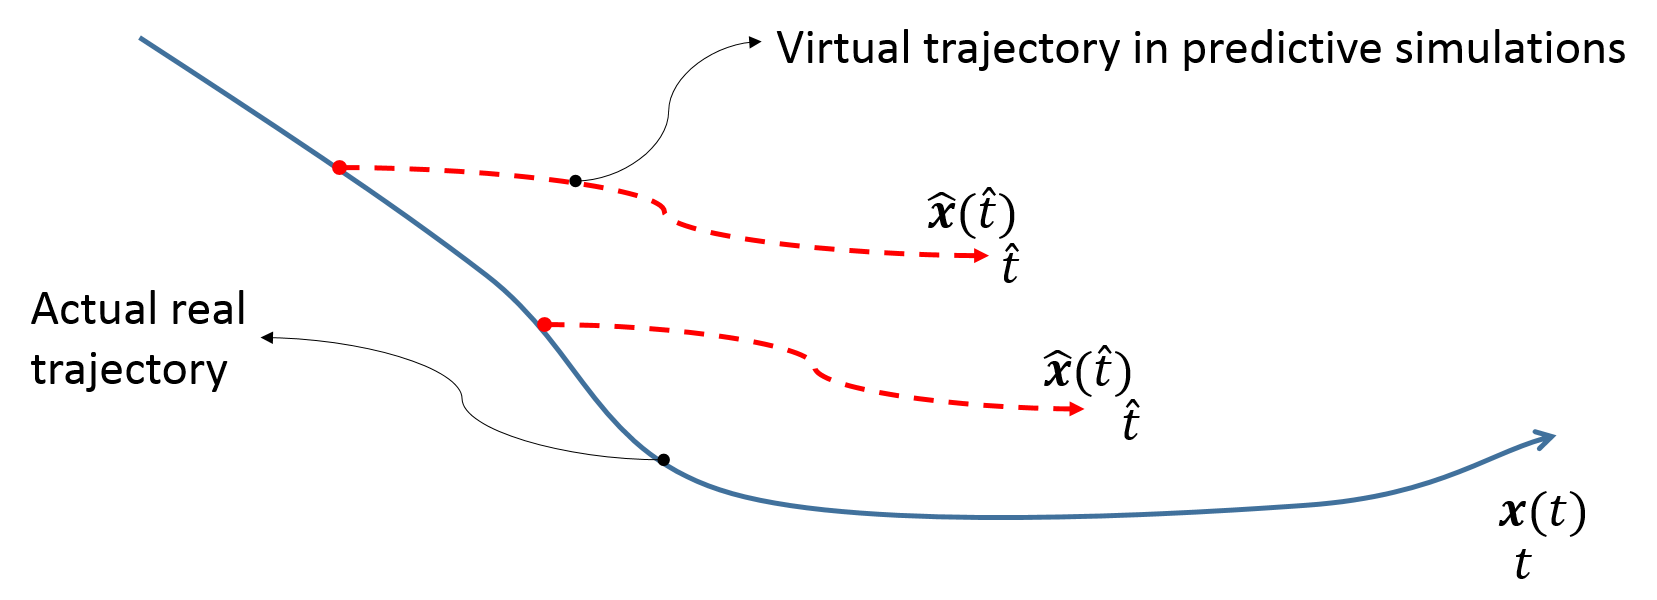
\includegraphics[width=0.8\textwidth]{rollouttrajs.png}
	\caption{Real trajectory and simulated virtual trajectory in the Rollout controller}
	\label{fig:rollouttrajs}
\end{figure}


\subsection{On a trajectory}
\label{sec:chat1}

Here a minimum time delay between a back-and-forth gear-shift sequence is derived for the situation where the robot has converged on a trajectory and is staying on the trajectory. In that case, it is assumed that both the simulation trajectory and the real system follow the same desired trajectory, see Fig. \ref{fig:costontrajrollout}.

\begin{figure}[H]
	\centering
		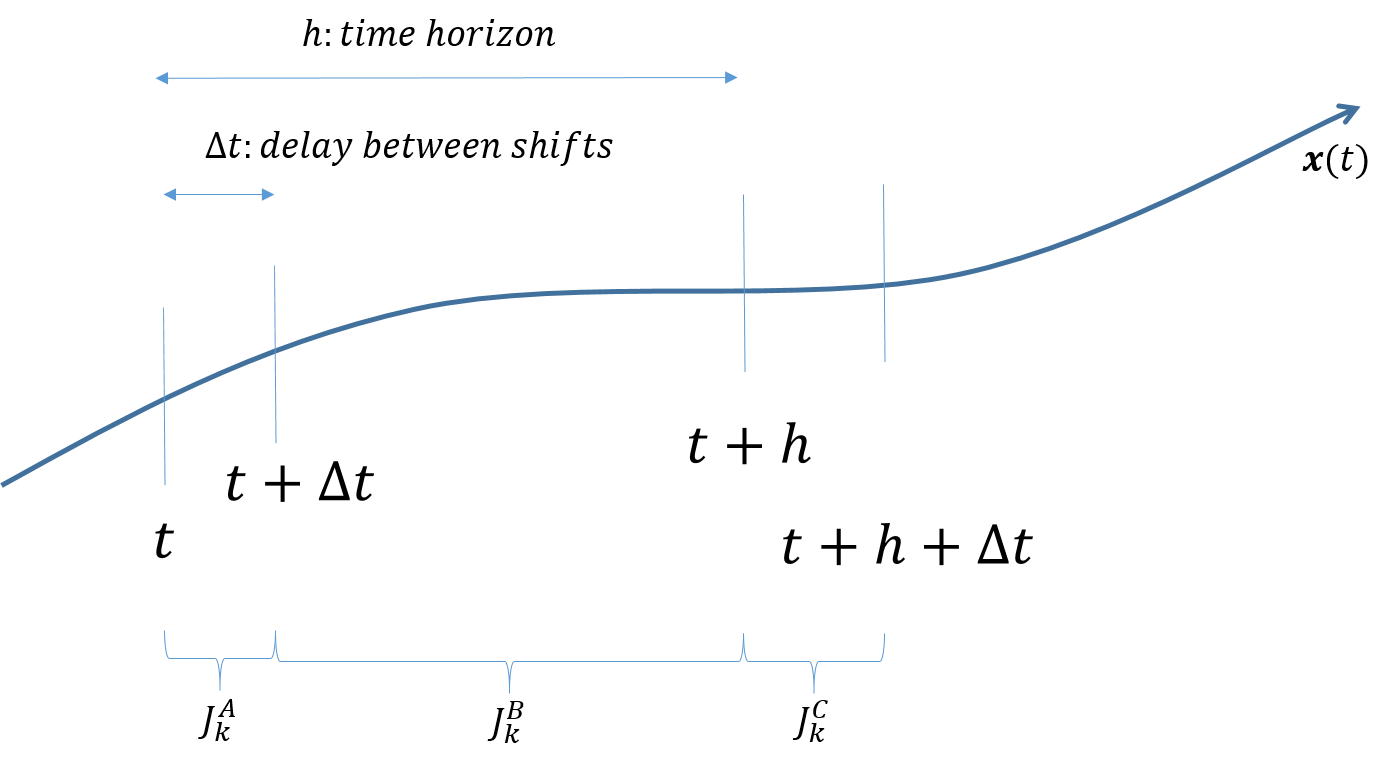
\includegraphics[width=0.90\textwidth]{costontrajrollout.png}
	\caption{Rollout controller behavior on a given trajectory}
	\label{fig:costontrajrollout}
\end{figure}

It can be shown that there is a minimum delay $\Delta t$ between a back-and-forth gear-shift sequence. Hence, no arbitrary fast chattering between gear-ratio (zeno behavior \cite{liberzon_switching_2003}) is possible. 

\paragraph{Proof} 

Without lost of generality, lets assume a gear shift sequence where the robot is first using mode $i$, then shift to mode $j$ at time $t$ and then shift back to mode $i$ at time $t+\Delta t$. If such a sequence happened while using the gear-ratio selection law given by eq. \eqref{eq:rolloutsimple}, then the following inequality must have been satisfied:
%
\begin{align}
i \rightarrow j  \quad\text{at time}\quad t          &\quad\Rightarrow\quad J_j(t) + Q < J_i(t)                  \\
j \rightarrow i  \quad\text{at time}\quad t+\Delta t &\quad\Rightarrow\quad J_i(t+\Delta t) + Q < J_j(t+\Delta t)
\end{align}
%
Then to simplify the notation, integral cost on the trajectory is given by the following value for each three sections of interest:
%
\begin{align}
J_k^A = \int_{t}^{t+\Delta t}{         C_k  d\hat{t}  }   \quad \quad
J_k^B = \int_{t+\Delta t}^{t+h}{       C_k  d\hat{t}  }   \quad \quad
J_k^C = \int_{t+h}^{t+\Delta t+h}{     C_k  d\hat{t}  }
\end{align}
%
Then it is possible to express the computed cost of predictive simulation done at $\Delta t$ time difference by the sum of a identical part and a different part:
%
\begin{align}
J_k(t)          &= \int_{t}^{t+h}{ C_k   d\hat{t} }  = J_k^A + J_k^B \\
J_k(t+\Delta t) &= \int_{t+\Delta t}^{t+\Delta t+h}{   C_k  d\hat{t}} = J_k^B + J_k^C
\end{align}
%
The difference between computed cost separated by $\Delta t$ is:
%
\begin{align}
\Delta J_k = J_k(t+\Delta t) - J_k(t) &= J_k^C - J_k^A
\end{align}
%
Now assuming there is an upper bound on instantaneous cost $C_k^{max}$, an upper bound also exist for the integral cost. Since the instantaneous cost is always positive definite, the integral cost cannot be negative. Hence:
%
\begin{align}
0 \leq J_k^C   \leq  C_k^{max} \Delta t \\
0 \leq J_k^A   \leq  C_k^{max} \Delta t 
\end{align}
%
The cost variation is thus bounded is this range:
%
\begin{align}
-C_k^{max} \Delta t  \leq \Delta J_k \leq C_k^{max} \Delta t
\end{align}
%
Hence the time evolution of computed cost can be bounded:
%
\begin{align}
J_j(t+\Delta t) \leq J_j(t)  + C_k^{max} \Delta t \\
J_i(t+\Delta t) \geq J_i(t)  - C_k^{max} \Delta t 
\end{align}
%
Finally it is possible to combine all those inequality, starting with the condition for the second gearshift:
%
\begin{align}
J_i(t)  - C_k^{max} \Delta t + Q \leq J_i(t+\Delta t) + Q &< J_j(t+\Delta t) \leq J_j(t)  + C_k^{max} \Delta t \\
J_i(t) + Q &\leq J_j(t)  + 2 C_k^{max} \Delta t \\
J_j(t) + 2 Q &\leq J_j(t)  + 2 C_k^{max} \Delta t \\
Q &\leq C_k^{max} \Delta t 
\end{align}
%
Hence resulting in the desired inequality relating instantaneous cost and time between gear-shift:
%
\begin{align}
\Delta t \geq \frac{Q}{C_k^{max}}
\end{align}
%
Note that if there is more than 2 discrete gear-ratio options, this analysis gives not insight about possible sequences of gear-shift during this interval, but still guarantee the minimum time for a full cycle (coming back to the starting gear-ratio).

\subsection{Arbitrary}
\label{sec:chat2}

